\documentclass{article}
\usepackage{graphicx}
\usepackage{subcaption}

\title{Report 6: Map Pattern}
\author{Nam Le}
\date{\today}

\begin{document}

\maketitle

\section{Implementation}
I implemented three parallel Map algorithms on GPU using Numba CUDA based on the slides:
\begin{enumerate}
    \item \textbf{Labwork 6a (Binarization)}: Calculated pixel grayscale value and applied threshold $\tau = 128$. Pixels above $\tau$ are set to 255 and below to 0.
    \item \textbf{Labwork 6b (Brightness Control)}: Added a constant delta (+67) to each RGB channel and clamped the result within $[0, 255]$.
    \item \textbf{Labwork 6c (Image Blending)}: Blended the original image with its horizontally flipped version using formula $Q(x,y) = c \cdot \Phi_1(x,y) + (1-c) \cdot \Phi_2(x,y)$ with weight $c = 0.67$.
\end{enumerate}

\section{Experimental Results}
The Map operations were executed with 2D block configurations $(8, 8)$, $(16, 16)$, and $(32, 32)$.

\begin{figure}[h]
    \centering
    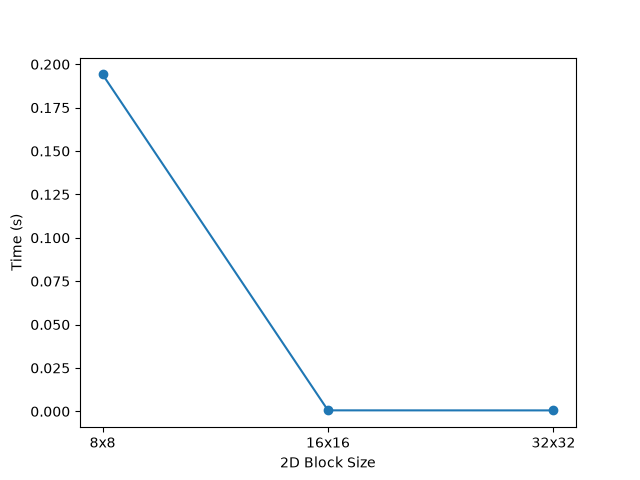
\includegraphics[width=0.7\textwidth]{map_block_size_vs_time.png}
    \caption{2D Block Size vs Execution Time for Map Pattern}
\end{figure}

\begin{figure}[h]
    \centering
    \begin{subfigure}[b]{0.45\textwidth}
        
\includegraphics[width=\textwidth]{binarization.jpg}
        \caption{Binarization ($\tau=128$)}
    \end{subfigure}
    \hfill
    \begin{subfigure}[b]{0.45\textwidth}
        
\includegraphics[width=\textwidth]{brightness.jpg}
        \caption{Brightness (+50)}
    \end{subfigure}
    
    \vspace{0.3cm}
    \begin{subfigure}[b]{0.6\textwidth}
        
\includegraphics[width=\textwidth]{blend.jpg}
        \caption{Image Blending ($c=0.6$)}
    \end{subfigure}
    \caption{Output images from Map pattern operations}
\end{figure}

\section{Discussion}
\begin{itemize}
    \item Map pattern algorithms perform 1-to-1 independent pixel operations, making them embarrassingly parallel.
    \item Block size $(8, 8)$ took around $0.125$s due to lower GPU core utilization.
    \item Block sizes $(16, 16)$ and $(32, 32)$ significantly reduced execution time to near $0.001$s as they provide much better warp occupancy.
\end{itemize}

\end{document}
